\chapter{MEASUREMENTS OF THE VISCOSITY OF THE QUASI-LIQUID LAYER AT THE SURFACE OF ICE-I$_\mathrm{h}$}\label{chap:QLL}

\begin{flushright}
\textit{''Why do snowflakes always fall as flat structures with six corners?''} \\
-Joannes Kepler (1611) \\
\end{flushright}

In the hydrodynamic friction regeime for a slider passing over an ice surface, three distinct forces contribute to the overall observed friction; the solid-liquid friction between the ice and quasi-liquid layer (QLL), the viscous shearing of the qll, and the solid-liquid friction between the qll and the slider. In Chapter \ref{chap:Friction}, we presented facet-dependent friction coefficients for the basal, prismatic, 14\degree~pyramidal, and secondary prism ice-I$_\mathrm{h}$ / water interfaces. In this chapter, we discuss the contribution of the viscous shearing of the qll at the basal and prismatic ice-I$_\mathrm{h}$ / vapor interface.



\section{Computational Methods}
TIP4P-Ice basal and prismatic ice-I$_\mathrm{h}$ primitive crystals were constructed following the procedure described in Chapter \ref{chap:Methods}. These primitive cells were then reoriented so that the desired crystal face was exposed to the $y$ axis, then replicated in the $x$ and $z$ dimensions to form large sheets. The sheets were then replicated in $y$ until the basal crystal was 12 bilayers thick, and the prismatic cyrstal was replicated to a width of approximately equal to the basal crystal. Dimensions and number of molecules in each system are found in Table \ref{tab:qll-method}.


\begin{table}[h]
\centering
\caption{SIZES OF THE VAPOR EXPOSED ICE-I$_\mathrm{h}$ / QUASI-LIQUID LAYER SIMULATIONS\label{tab:qll-method}}
\begin{tabular}{r|c|ccc}
\hline
\hline
 Interface & $N_\mathrm{ice}$ & $L_x$ & $L_y$ & $L_z$ \\
\hline
Basal  $\{0001\}$                           & 46,080 & 185.24 & 44.04 & 186.06 \\
Prismatic  $\{10\bar{1}0\}$            & 55,000 & 192.47 & 49.14 & 181.61\\
\hline
\hline
\end{tabular}
\begin{flushleft}
Box dimensions are given in \AA.
\end{flushleft}
\end{table}


The $y$-dimension of the simulation box was then set to 300~\AA~ to allow for a surface premelt to form, and each system was equilibrated to 265~K~. The resulting systems exposed two interfaces, one toward positive $y$ and the other towards negative $y$. The equilibration was conducted under a constant pressure and temperature integrator, allowing the $x$ and $z$-dimensions of the simulation cell to relax and alleviate any crystal strain. Following this the systems were then equilibrated under a constant volume and temperature integrator, and lastly under a constant volume and energy integrator. During these simulations, the width of the crystal (in the $y$-dimension) was monitored to ensure no appreciable crystal melt occurred.

Once equilibrated, a shear stress was applied only to molecules within the QLLs using the velocity shearing and scaling variant of reverse non-equilibrium molecular dynamics described in Chapter \ref{chap:Methods}.\cite{Kuang2012} The VSS-RNEMD exchange regions were defined to incorporate molecules from both the top and bottom interfaces, as seen in Figure \ref{fig:qll-rnemd}. Both the tangential density and tetrahedrality profiles were used to determine the $y$-width of the exchange VSS-RNEMD regions. In Chapter \ref{chap:Str}, we found the tetrahedrality at the Gibbs dividing surface for ice-I$_\mathrm{h}$ / water interfaces to be $q^{Gibbs} \sim$0.84. Here, we have used $q^{Gibbs}$ as the cutoff value between the QLL and the ice. All molecules with $q < q^{Gibbs}$ are denoted as QLL molecules, while those with $q > q^{Gibbs}$ are denoted to be ice. This cutoff coincides with a minimum in the tangential density profiles, as seen in the top and bottom panels of Figure \ref{fig:qll-rhoq}.


\section{Distance Dependence of Viscosity from the Ice Surface}
As seen in Figure \ref{fig:qll-rhoq}, the QLLs at the surface of the
basal and prismatic crystals form a bilayer. Following Neshyba
\textit{et al.}, we denote the following definitions; molecules within
the ice are labeled as $\mu_{i}$, where each $i$ denotes a unique
density peak in the ice, molecules in the QLL layer closer to the ice
are labeled as $\epsilon_{2}$, and molecules in the outter portion of
the QLL bilayer are labeled as $\epsilon_{1}$.\cite{Neshyba2009} Due
to their relative distances from the underlying crystal, molecules
within layers $\epsilon_{2}$ and $\epsilon_{1}$ experience vastly
different local environments. Water molecules within $\epsilon_{2}$
located closer to the ice experience significantly more drag than
those closer to the vapor. Therefore, we expect a noticeably different
sheaer viscosity for the molecules located in $\epsilon_{2}$ and
$\epsilon_{1}$. 

The shear viscosity, $\eta$, of the QLL can be determined using the linear
constitutive relation for a shear stress imposed across a liquid.
\begin{equation}\label{eq:qll-visco}
j_z(p_x) = \eta \frac{\partial v_x}{\partial z}
\end{equation}
Since the QLLs are composed of multiple layers of varying densities
and local structures, their response to the shear stress may vary. Due
to this, we have computed $\eta$ for thin slices of $y$ through the
QLLs as seen in Figure \ref{fig:qll-vx}.

\begin{figure}
\includegraphics[width=\linewidth]{Figures/qll-vx}
\caption{\label{fig:qll-vx} Shearing profiles of the basal QLLs for
  molecules close to the underlying ice surface ($\epsilon_{2}$) and
  molecules closer to the vapor ($\epsilon_{1}$). }
\end{figure}                


\begin{figure}
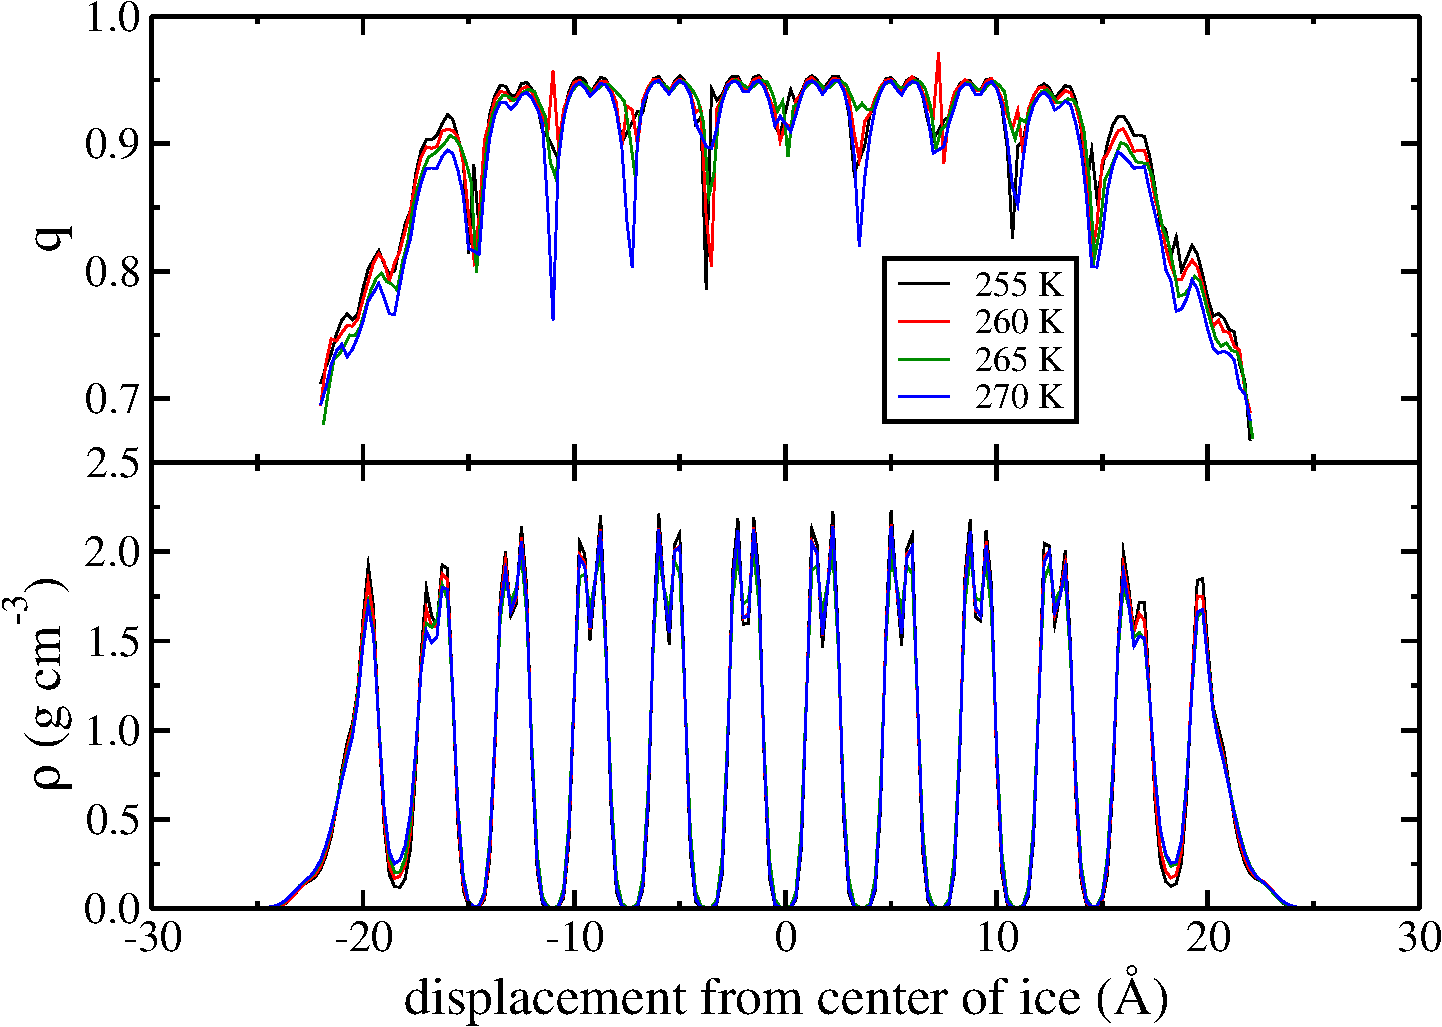
\includegraphics[width=\linewidth]{Figures/basal_rhoq}
\caption{\label{fig:basal_rhoq} Shearing profiles of the basal QLLs for
  molecules close to the underlying ice surface ($\epsilon_{2}$) and
  molecules closer to the vapor ($\epsilon_{1}$). }
\end{figure}                


\begin{figure}
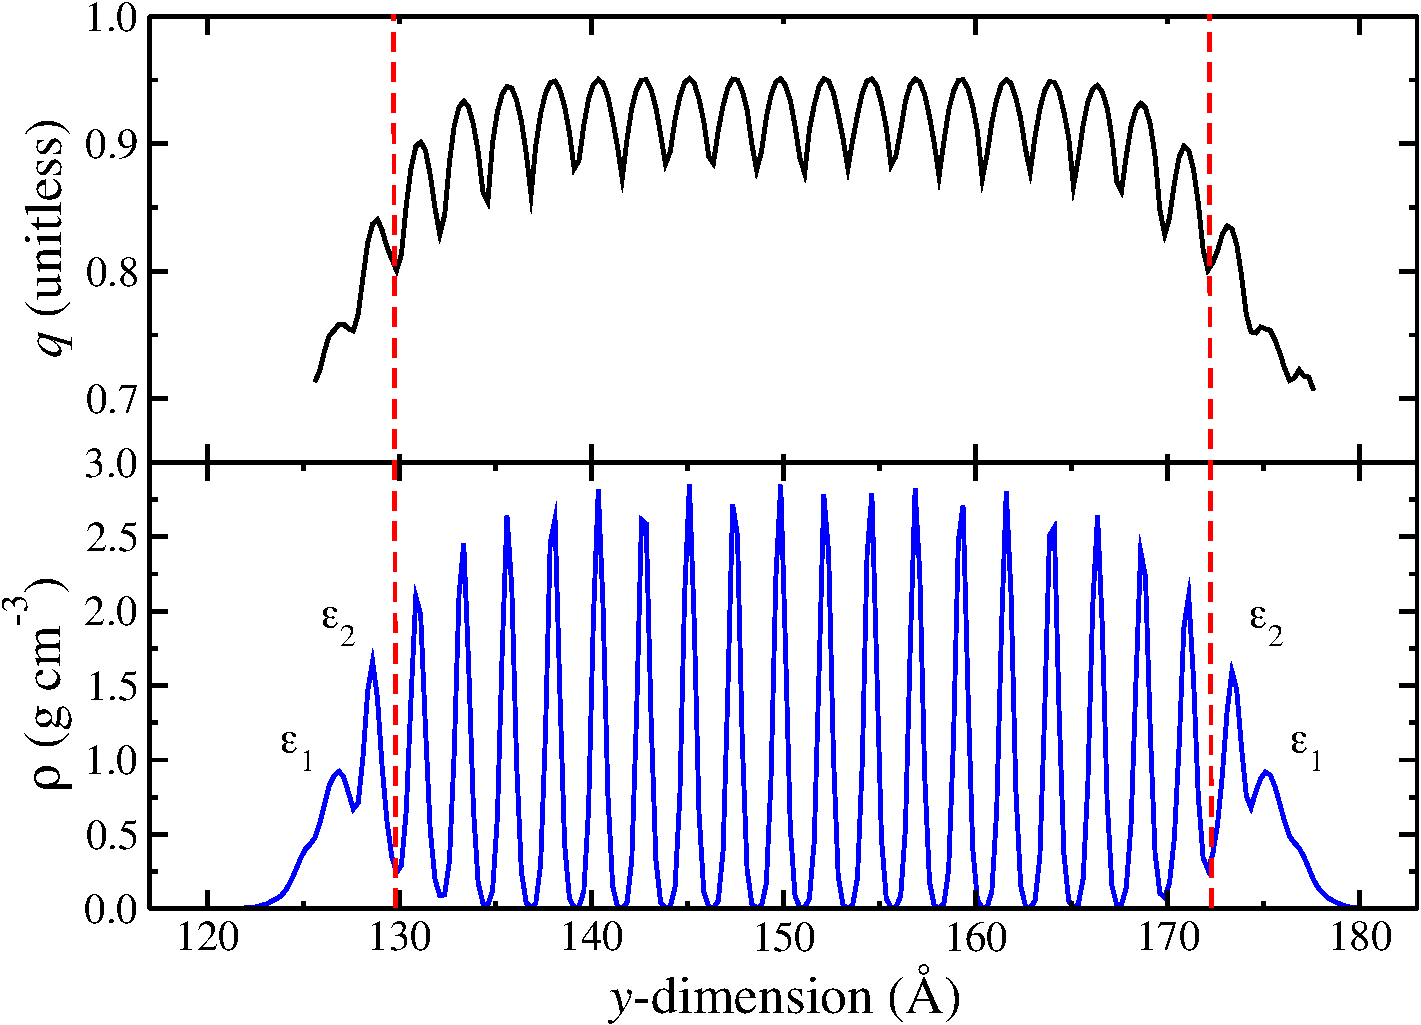
\includegraphics[width=\linewidth]{Figures/prism_rhoq}
\caption{\label{fig:prism_rhoq} Shearing profiles of the basal QLLs for
  molecules close to the underlying ice surface ($\epsilon_{2}$) and
  molecules closer to the vapor ($\epsilon_{1}$). }
\end{figure}                



Previous estimates of the viscosity of the quasi-liquid layer (QLL) on the surface of
ice have come from the Stoke's-Einstein relation, which relates the
diffusion of the surface molecules to the viscosity. However,
molecules at the surface of ice which are transitory in the vapor
phase can skew the results, as their mean-square displacements will be
much larger than those in the condensed phase. Due to this, our
estimates which are much less sensative to temporary vapor phase
trajectories, provide better computational estimates of the viscosity
of the qll.

Neshyba \textit{et al.} studied the basal qll using the six site water
model developed by Nada and van der Eerden. Neshyba investigated water
accommodation and sublimation events, focusing on the underlying
mechanisms for the events to occur. They observed long rotational and
thermal relaxation of incident gas phase water molecules as they
condensed into the qll and into the ice. \cite{Neshyba2009} 


% In a recent review of Ice Surfaces, Mary Jane Shultz posed numerous
% open questions about the qll, such as what is the growth mechanism,
% relative energies of various vaces are not well understood, what is
% the impact of face termination on ice surface energy and reactivity,
% what defintion is relevant for the qll, at what temperature does the
% qll from, what is the nature of the qll?

2017 PNAS paper by M. Alejandra Sanchez \textit{et al.} provides
experimental (surface-specific vibrational sum frequency generation
spectroscopy)  and theoretical (molecular dynamics simulations with
the TIP4P/Ice model)
evidence that the qll formation occurs
bilayer-by-bilayer. Observed for the basal face and the secondary prism. 

% Determination of Surface Tension-to-Shear VIscosity Ratio for
% Quasiliquid layers on Ice Crystal Surfaces.
%   K. Murata, H. Asakawa, K. Nagashima, Y. Furukawa, G. Sazaki
%   PRL 115 (2015) 256103
Using laser confocal microscopy in conjunction with an inverted
optical microscope, Murata \textit{et al.} have recently measured the
characteristic-velocity (\textit{i.e.} the surface tension-to-shear
viscosity ratio) of two distinct wetting morphologies of QLLs on the
basal surface of ice at -0.2 degrees Celcius and a pressure of 578.9
Pa.\cite{Murata2015} They observed a partial wetting QLL, described as
a bulk liquid droplet (BLD), as well as a complete wetting state,
described as a thin liquid layer (TLL). The characterstic-velocity of
the BLDs was determined from relaxation modes of their contact lines,
which was observed to decay with single exponential behavior according
to
\begin{equation}
u_q = u_q(0) exp\Bigg(-\frac{V^* \theta^3 q}{3l}t\Bigg)
\end{equation}
where $q$ is the wave vector for the perturbing mode for the
relaxation of the amplitude of the contact line and $u_q(0)$ being the
initial amplitude of the mode. Here, $V^* = \gamma / \eta$ is the
characteristic velocity and $\theta$ is the contact angle the BLD makes
with the ice surface ($\sim$ 2 degrees). Lastly, the logarithmic factor
$l=ln(L/a)$ is a cutoff parameter which helps avoid
singularities. From this fit, they obtained $V^* = 2 \pm 1$ m/s, which
is about an order of magnitude smaller than that of bulk water, 42.21
m/s.

Murata \textit{et al.} also investigated the spreading dynamics of the
BLD-QLLs, during the transformations to TLL-QLLs. The radii of the
spreading BLD-QLLs were fit to a power law
\begin{equation}
r = L (\frac{4S}{3Ll \eta})^{1/4}(t+t_0)^{1/4}.
\end{equation}
Here, $S$ is the spreading coefficient, and $t_0$ captures the initial
state of the droplet. As the QLL transitions from the BLD
drpolet-shape to the TLL pancake-shape, the volume must be
conserved. From this conservation, Murata \textit{et al.} estimated
the thickness of the TLLs as 9 $\pm$ 3 nm.

Lastly, Murata \textit{et al.} have obtained the characterstic
velocity of the TLLs in the same way as the BLDs. However, here the
hydrodynamic dissipation is not located at the wedge of the droplet
like in the BLD case, but instead the dissipation occurs within the
fluid of the pancake-shape object itself. Due to this, a slightly
different expression for the viscious force must be used, and the
resulting characteristic velocity was found to be $V^* = 0.2 \pm 0.1$
m/s, about 200 times smaller than that of bulk water. This seems to
imply a dependence on the characterstic velocity to the QLLs contact
area and distance from the surface. The BLD droplet-shaped QLLs (where
the QLL is only partially wets the surface and a larger amount of the
QLL resides further from the surface), were found to have a
characterstic velocity of about an order of magnitude larger than the
more completely wetting state, where more of the QLL resides closer to
the surface.

It is interesting to note that the surface tension of the BLD/air
interface ($\gamma_t$) is approximately equal to the TLL/air interface
surface tension ($\gamma_b$), as there is observed coexistence of both
forms of QLLs at the same time. Therefore, the discrepency in $V^*$
can be primarily attributed to the shear viscosity of the QLL phase.
 
% end Murata2015


Discuss widths of qll by experimental groups. Probing different
measures of the qll gives different widths at different
temperatures. Give a quick summary of the kinds of experiments and
what their findings were for qll widths.




Break down of stoke's-einstein relation for viscosity. \cite{Chen2006,
  Tarjus1995,Bordat2003,Kumar2007}
